\newgeometry{margin=0.5in}

% Reinstate this until they yell at you; it's ridiculous
% Here in 2018 because I already messed up other stuff.
% \thispagestyle{empty}

\textbf{Name:} \rule{5cm}{1pt} \hfill \textbf{Student No:} \rule{5cm}{1pt} \\

\bigskip\noindent \hfill {\large {\bf BIOLOGY 3SS3}, C01,
	% Version \testver
	DEFERRED
} \hspace*{\fill} \\
DAY CLASS  \hfill Jonathan Dushoff \\
Test duration: 2 hours \hfill June 2018

{\small

\medskip\noindent THIS TEST INCLUDES {\bf 40 QUESTIONS} and \textbf{\pageref{LastPage} PAGES}. YOU ARE RESPONSIBLE FOR ENSURING THAT YOUR COPY OF THE PAPER IS COMPLETE. BRING ANY DISCREPANCY TO THE ATTENTION OF YOUR INVIGILATOR. 

\begin{itemize}
\item McMaster standard calculator (Casio FX-991 MS or MS Plus) is permitted for this exam.
\item Print your name and student number on the front page of this exam paper.
\item Answer questions 1-40 on the \textbf{optical scan sheets}.  Carefully read the following instructions.
\end{itemize}
\hrule
\bigskip\textbf{SCAN SHEET INSTRUCTIONS:} 
IT IS YOUR RESPONSIBILITY TO ENSURE THAT THE ANSWER SHEET IS PROPERLY COMPLETED. YOUR EXAMINATION RESULT DEPENDS UPON PROPER ATTENTION TO THESE INSTRUCTIONS.

The scanner, which reads the sheets, senses the bubble-shaded areas by their non-reflection of light.  A heavy mark must be made, completely filling the circular bubble, with a HB pencil.  Marks made with a pen or felt-tip marker will NOT be sensed.  Erasures must be thorough or the scanner may still sense a mark.  Do NOT use correction fluid on the sheets.  Do NOT put any unnecessary marks or writing on the answer sheet.

\begin{enumerate}

\item On side 1 (red side) of the form, in the top box, in pen, print your student number (NOTE: 9 digits), name, course name, section number, instructor name and date in the spaces provided.  Then you MUST write your signature in the space marked SIGNATURE.

\item In the second box, with a pencil, mark your student number, exam version number, and course section number in the space provided and fill in the corresponding bubble numbers underneath.

\item To indicate your answers, mark only ONE choice from the alternatives (1,2,3,4,5 or a,b,c,d,e) provided for each question.  The question number is to the left of the bubbles.  Make sure that the number of the question on the scan sheet is the same as the question number on the test paper.

\item Pay particular attention to the Marking Directions on the form.

\item Begin answering questions using the first set of bubbles, marked ``1''.

\end{enumerate}

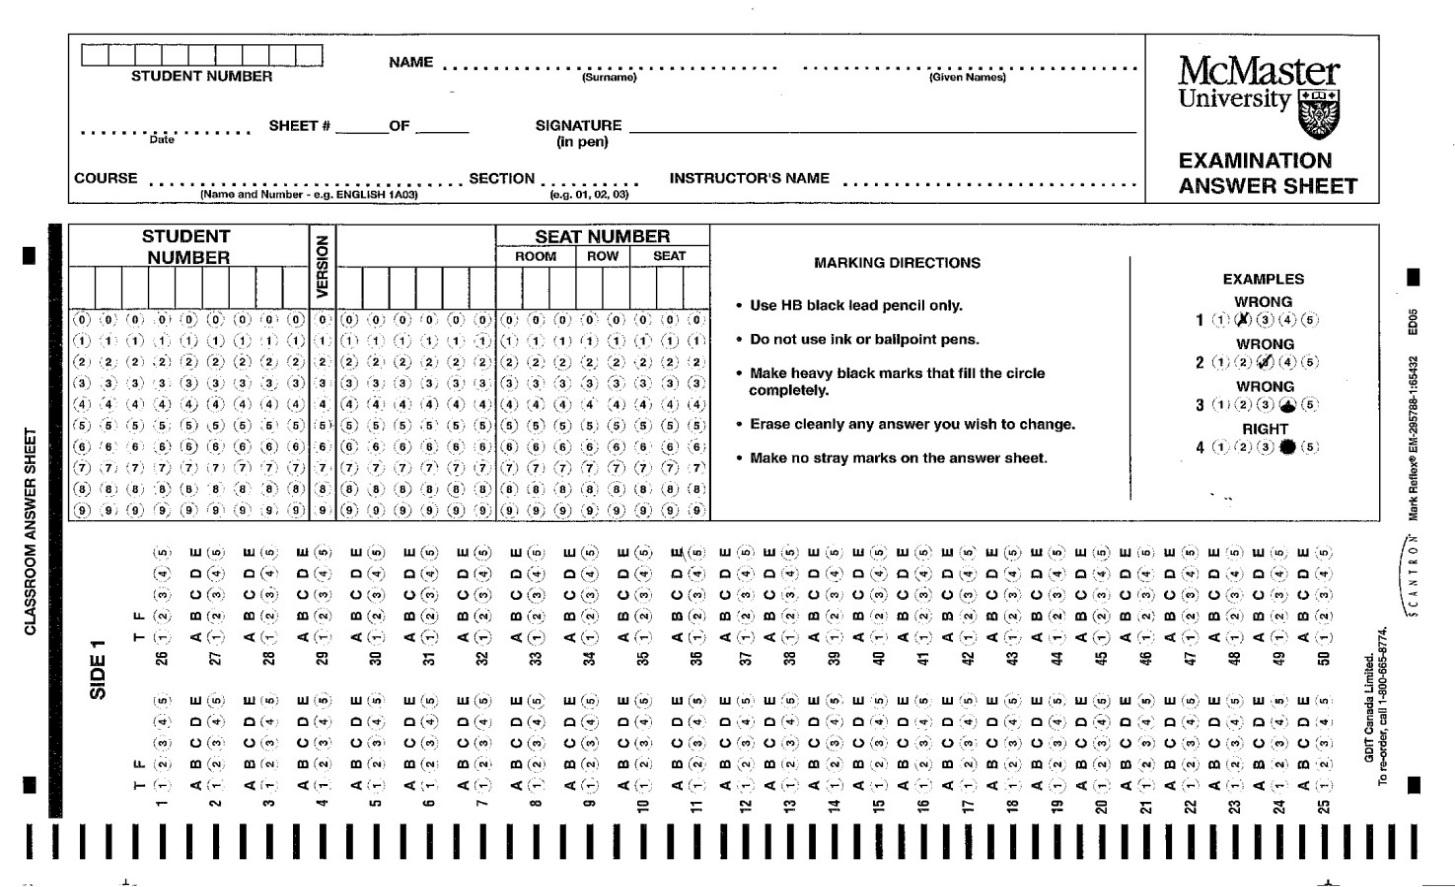
\includegraphics[height=2in]{scantron.jpg}

\center{{\large {\it Good luck!}}}
}


